\subsection{Subgraph Algorithms}
\label{sec:subgraph-vertex-minor-alg}

\begin{fact}
Given a finite graph $G = (V,E)$, we can decide whether it is the vertex minor of some circle graph in linear time, with respect to the number of vertices and edges of $G$.
\end{fact}

\begin{proof}
By Theorem \ref{thm:circle-graph-closed-vertex-minor}, circle graphs are closed under vertex minors. Thus to decide whether $G$ is a vertex minor of some circle graph is equivalent to deciding whether $G$ is a circle graph. \cite{paul2025circlegraphsrecognizedlinear} presents a linear time algorithm for this, using PC-trees \cite{paul2025circlegraphsrecognizedlinear}.
\end{proof}

Note that by Theorem \ref{thm:cgraph-vertex-minor-cgrid}, the above is equivalent to deciding if $G$ is a vertex minor of some comparability grid. If we restrict our attention to deciding if $G$ is an induced subgraph of some comparability grid, we obtain similar results.

\begin{fact}
\label{fact:perm-graph-iff-subgraph-cgrid}
A finite graph $G$ is an induced subgraph of a comparability grid if and only if $G$ is a permutation graph.
\end{fact}

\begin{proof}
This is just a restatement of Fact \ref{fact:tuple-construction}.
\end{proof}

\begin{lemma}
\label{lemma:permutations-mod-reverse-complement}
Let \(R_k\) be the number of permutations of \([k]\), modulo the equivalence
relation generated by reverse-complement
$
    \pi^{rc}(i) := k+1-\pi(k+1-i)
$.
Then
\begin{align}
    R_k
    =
    \frac{k!+2^{\lfloor k/2\rfloor}\lfloor k/2\rfloor!}{2}.
\end{align}
\end{lemma}

\begin{proof}
The operation \(\pi\mapsto \pi^{rc}\) has order \(2\), so each equivalence
class has size \(1\) or \(2\). By Burnside's lemma, the number of equivalence
classes is the average number of permutations $\pi$ fixed by the two operations:
the identity operation and reverse-complement. Hence
\begin{align}
    R_k
    =
    \frac{
        \#\{\text{$\pi$ fixed by the identity}\}
        +
        \#\{\text{$\pi$ fixed by reverse-complement}\}
    }{2}.
\end{align}
The identity fixes every permutation, so the first term is \(k!\).

It remains to count the permutations fixed by reverse-complement. Such a
permutation satisfies \(\pi=\pi^{rc}\), which means
\begin{align}
    \pi(i)
    =
    k+1-\pi(k+1-i).
\end{align}
Equivalently,
$
    \pi(i)+\pi(k+1-i)
    =
    k+1.
$
Thus the positions come in symmetric pairs
\(\{1,k\},\{2,k-1\},\dots\), and the values also come in symmetric pairs
\(\{1,k\},\{2,k-1\},\dots\). There are \(\lfloor k/2\rfloor\) such
position-pairs and \(\lfloor k/2\rfloor\) such value-pairs.

To build a reverse-complement-fixed permutation, first match the
position-pairs with the value-pairs. This can be done in
\(\lfloor k/2\rfloor!\) ways. Then, for each matched pair, choose which of
the two values goes in the smaller position. This gives
\(2^{\lfloor k/2\rfloor}\) choices. If \(k\) is odd, the middle position is
forced to take the middle value, so it gives no extra choice. Therefore the
number of permutations fixed by reverse-complement is
\begin{align}
    2^{\lfloor k/2\rfloor}\lfloor k/2\rfloor!.
\end{align}
Substituting into Burnside's lemma gives the desired result.
\end{proof}

We remark that, for $k\geq 3$, $R_k$ is strictly smaller than $k!$. For $k \geq 10$, $R_k$ is strictly smaller than the number of connected circle graphs with $k$ vertices. The latter is given by sequence $A156808$ in the Online Encyclopedia of Integer Sequences \cite{OEIS_A156808}. 

We would like this number to be as small as possible so that we may more easily conduct a census of all $k$-vertex subgraphs of $\CGrid$. For example, we may be interested in a census of the degree sequences of all $k$-vertex subgraphs. The following fact and lemma show that we may do this in $O(R_k \cdot k \log k)$ time.

\begin{fact}
In order to enumerate every $k$-vertex subgraph of any $\CGrid$, it suffices to enumerate $R_k$ objects.
\end{fact}

\begin{proof}
This follows from Fact \ref{fact:perm-graph-iff-subgraph-cgrid} and Lemma \ref{lemma:permutations-mod-reverse-complement}.
\end{proof}

\begin{lemma}
Let \(\pi\in S_k\). We can compute the degree sequence of \(H(\pi)\) in
\(O(k\log k)\) time.
\end{lemma}

\begin{proof}
Recall that \(ij\in E(H(\pi))\) iff
\begin{align}
    (i-j)(\pi(i)-\pi(j))>0.
\end{align}
Thus the degree of vertex \(i\) splits into a {\color{red}forward contribution} and a {\color{blue}backward contribution}:
\begin{align}
    \deg(i)
    =
    {\color{red}\#\{j<i:\pi(j)<\pi(i)\}}
    +
    {\color{blue}\#\{j>i:\pi(i)<\pi(j)\}}.
\end{align}

A Fenwick tree is a well-known data structure that stores counts over the values
\([k]\). It supports two operations in \(O(\log k)\) time: inserting a value
\(t\), and querying how many inserted values are at most \(t\). Thus, after
inserting some subset of values, a query at \(t\) returns
\begin{align}
    \#\{\text{inserted values } \leq t\}.
\end{align}

We compute the {\color{red}forward term} by scanning \(\pi\) left to right
with a Fenwick tree. At step \(i\), the tree stores the values
\(\pi(1),\dots,\pi(i-1)\). Therefore a query at \(\pi(i)-1\) gives
\begin{align}
    {\color{red}
    L_i=\#\{j<i:\pi(j)<\pi(i)\}}.
\end{align}
Then insert \(\pi(i)\). The {\color{blue}backward term} is analogous, but we scan from right to left. Each scan performs \(O(k)\) Fenwick-tree updates and queries, each taking \(O(\log k)\) time. Hence the total runtime is \(O(k\log k)\).
\end{proof}

\begin{figure}[H]
\[
\begin{minipage}{0.3\textwidth}
\centering
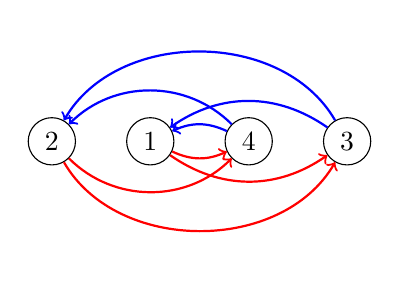
\begin{tikzpicture}[
    scale=1.25,
    vertex/.style={circle, draw, inner sep=1.5pt, minimum size=6mm},
    rededge/.style={->, color=red, thick},
    blueedge/.style={->, color=blue, thick}
]
    \node[vertex] (n1) at (0,0) {$2$};
    \node[vertex] (n2) at (1,0) {$1$};
    \node[vertex] (n3) at (2,0) {$4$};
    \node[vertex] (n4) at (3,0) {$3$};

    \draw[rededge] (n1) to[bend right=45] (n3);
    \draw[rededge] (n1) to[bend right=60] (n4);
    \draw[rededge] (n2) to[bend right=25] (n3);
    \draw[rededge] (n2) to[bend right=35] (n4);

    \draw[blueedge] (n3) to[bend right=45] (n1);
    \draw[blueedge] (n3) to[bend right=25] (n2);
    \draw[blueedge] (n4) to[bend right=60] (n1);
    \draw[blueedge] (n4) to[bend right=35] (n2);
\end{tikzpicture}
\end{minipage}
\hfill
\begin{minipage}{0.3\textwidth}
\centering
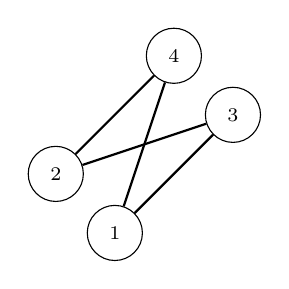
\begin{tikzpicture}[
    scale=0.75,
    gridline/.style={gray!25, very thin},
    vertex/.style={circle, draw, fill=white, inner sep=1.5pt, minimum size=7mm},
    edge/.style={thick}
]
    \node[vertex] (v1) at (1,2) {\scriptsize \(2\)};
    \node[vertex] (v2) at (2,1) {\scriptsize \(1\)};
    \node[vertex] (v3) at (3,4) {\scriptsize \(4\)};
    \node[vertex] (v4) at (4,3) {\scriptsize \(3\)};

    \draw[edge] (v1) -- (v3);
    \draw[edge] (v1) -- (v4);
    \draw[edge] (v2) -- (v3);
    \draw[edge] (v2) -- (v4);
\end{tikzpicture}
\end{minipage}
\]
\caption{For \(\pi=2143\), the left figure shows the {\color{red}forward} and {\color{blue}backward} contributions to the degree sequence. The right figure shows $H(\pi)$.}
\label{fig:fenwick-tree-example}
\end{figure}

With these results in hand, we can conduct a census of $k$-vertex subgraphs relatively easily. For example, we can enumerate all $9$-vertex subgraphs of $\CGrid$ that themselves have the $\Grid_{3 \times 3}$ as an induced subgraph. From this, we obtain that the $\CGrid$ is not an induced subgraph of any comparability grid (Fact \ref{fact:grid-3-times-3-not-subgraph}). On the other hand, we obtain two interesting 